\chapter[INTERSCITY]{INTERSCITY}
\label{chapter:interscity}

O InterSCity é uma plataforma de cidades inteligentes nascida a partir de
estudos científicos que buscavam endereçar os principais desafios encontrados
no desenvolvimento de infraestruturas de cidades inteligentes \cite{nof2016}.
Está licenciado sob
MPLv2\footnote{\url{www.mozilla.org/en-US/MPL/2.0/}}, foi construído com a
utilização da arquitetura de microsserviços -
MSA\footnote{\url{microservices.io/}}, e tem como principal objetivo prover os
serviços e integrações necessárias para a construção de aplicações de cidades
inteligentes complexas \cite{delesposte2017}. Baseando-se no desenvolvimento
colaborativo e na utilização de tecnologias software livre, o projeto é
desenvolvido com a ajuda de diversos colaboradores, que utilizando práticas
ágeis, atuam na manutenção e evolução da plataforma ao longo do tempo
\cite{delesposte2017}.

A maior parte dos microsserviços\footnote{Os termos microsserviços, módulos, e
componentes, serão utilizados intermitentemente, mas apresentando o mesmo
significado.} da plataforma foram escritos em Ruby on Rails\footnote{\url{rubyonrails.org/}},
seguindo padrões que priorizam extensibilidade e qualidade, e levando em conta
princípios\footnote{Os princípios seguidos pelo InterSCity são apresentados no
Apêndice \ref{appendix:principles}} que levaram a uma arquitetura madura,
robusta e extensível. A partir de experimentos feitos foi possível conferir
o quão promissor é a performance e a escalabilidade do InterSCity, provando-se
capaz de lidar com cenários reais de cidades inteligentes \cite{delesposte2017}.
O projeto encontra-se hospedado no
Gitlab\footnote{\url{gitlab.com/smart-city-software-platform}},
onde é possível ter acesso ao código fonte, documentação, e um exemplo de
cliente que ilustra o uso da plataforma.

\section{ARQUITETURA}
\label{sec:architecture}

O InterSCity é composto por uma arquitetura de microsserviços distribuída,
que possibilita armazenamento, análise, processamento, composição e
integração de dados de recursos de cidades inteligentes. Estes microsserviços
são desacoplados entre si, e se comunicam através de requisições REST e
passagem de mensagem, modelo importante em contextos de concorrência por conta
do isolamento provido \cite{armstrong2003}. No InterSCity a troca de mensagem
é feita com auxílio do \textit{broker} de mensagens
RabbitMQ\footnote{\url{www.rabbitmq.com/}}, através do padrão de projeto
PubSub\footnote{\url{xmpp.org/extensions/xep-0060.html}}.

\begin{figure}
  \centering
    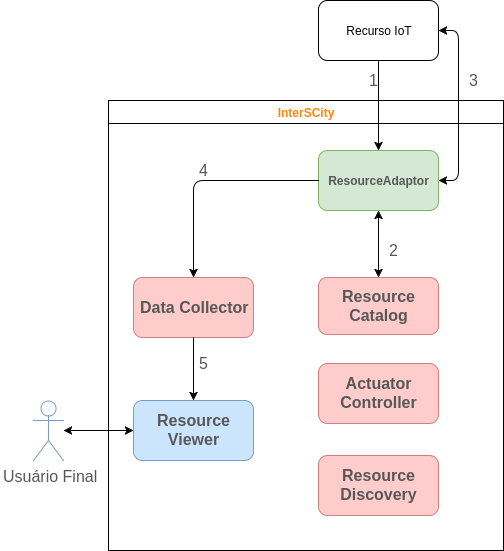
\includegraphics[scale=0.5]{figuras/interscity_flow.png}
  \caption{Ciclo de vida de um recurso IoT no InterSCity. Baseado em: \citeonline{delesposte2017}.}

  \label{fig:interscity-lifecycle}
\end{figure}

A Figura \ref{fig:interscity-lifecycle} ilustra o ciclo de vida típico de um
recurso IoT na plataforma. Inicialmente um recurso IoT (1) faz um pedido de
registro na plataforma via Resource Adaptor, que (2) cadastra o recurso no
microsserviço Resource Catalog (3) e informa o UUID
(identificador único) que será utilizado internamente desse passo em diante.
Após, a comunicação entre o Resource Adaptor e o dispositivo IoT terá
continuidade, mas (4) os dados terão como destino o módulo Data Collector,
que armazenará as informações. Por fim, (5) as informações contidas no
Data Collector são disponibilizadas, podendo ser apresentadas para um usuário
final via Resource Viewer, ou consumidas por uma aplicação cliente.

Os microsserviços do InterSCity têm responsabilidades atômicas e bem
definidas, princípio chave para que a plataforma contemple requisitos funcionais
e não-funcionais. O microsserviço \textbf{Resource Adaptor} é o grande
responsável pela comunicação entre os dispositivos IoT e a plataforma,
funcionando como um mediador durante as requisições \cite{delesposte2017}.

O \textbf{Data Collector} e o \textbf{Resource Catalog} tem papéis parecidos,
mas enquanto o primeiro gerencia e armazena dados históricos de medições dos
dispositivos, o segundo tem o papel de gerenciar e armazenar o registro dos
dispositivos na plataforma \cite{delesposte2017}.

\begin{figure}
  \centering
    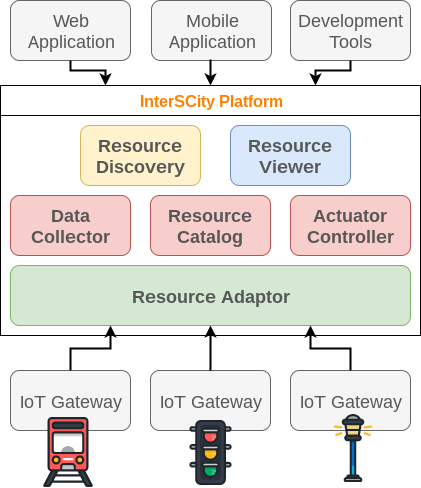
\includegraphics[scale=0.5]{figuras/interscity_architecture.png}
    \caption{Arquitetura completa do InterSCity. Fonte: \citeonline{delesposte2017}.}
  \label{fig:interscity-architecture}
\end{figure}


O \textbf{Resource Viewer} e o \textbf{Resource Discovery}, por outro lado,
são similares por manipularem e utilizarem o Data Collector e o Resource
Catalog em sua execução. O Resource Viewer tem como objetivo apresentar ao
usuário final os dados dos recursos, enquanto o Resource Discovery provê uma API
 de busca por dispositivos disponíveis, possibilitando o uso de filtros
\cite{delesposte2017}. Por fim, o \textbf{Actuator Controller} provê serviços
para requisições nos recursos IoT atuadores registrados na plataforma,
armazenando os dados e possibilitando auditoria \cite{delesposte2017}. A Figura
\ref{fig:interscity-architecture} trás uma visão geral da arquitetura, com todos
os microsserviços reunidos, apresentando as fronteiras entre a plataforma,
aplicações clientes e dispositivos.

\section{GERÊNCIA DE CONFIGURAÇÃO E DEPENDÊNCIAS}

Outro aspecto que recebe atenção no desenvolvimento do InterSCity é a gerência
de configuração, que atualmente utiliza tecnologias que reduzem o esforço
desnecessário, promovem o isolamento entre a plataforma e o ambiente hospedeiro
e aumentam a segurança no desenvolvimento. A gerência de configuração do
InterSCity é guiada por conteinêres do
Docker\footnote{\url{https://www.docker.com/}}, e cada microsserviço e
dependência externa (como o RabbitMQ) são executados em
conteinêres separados. O desenvolvimento da plataforma também faz extenso
uso do Git\footnote{\url{https://git-scm.com/}}, de modo que a
configuração de um ambiente para execução do InterSCity tenha como
pré-requisitos somente estes dois projetos: Docker e Git.

Cada microsserviço da plataforma tem seu próprio repositório, permitindo que
evoluam de maneira distribuída. Com o propósito de ajudar no desenvolvimento,
o InterSCity apresenta um repositório principal chamado
\textit{dev-env}\footnote{\url{https://gitlab.com/smart-city-software-platform/dev-env}},
que funciona como \textit{repositório mestre}, sendo os repositórios dos
microsserviços da plataforma submódulos pertencentes ao \textit{dev-env}.

\section{PROPOSTA E METODOLOGIA}

Atualmente o InterSCity está em constante desenvolvimento, e embora não conte
com uma camada de processamento de dados ideal, certo esforço culminou em um
serviço de processamento provisório, que será utilizado como base para o
desenvolvimento da nova arquitetura. Houve ainda a troca de tecnologia de banco
de dados no microsserviço Data Collector, que passou do Postgres (tecnologia
SQL) para o MongoDB (tecnologia NoSQL), troca importante na busca por uma maior
elasticidade no volume de dados. A equipe do InterSCity nomeou a camada
provisória de \textbf{Data Processor}, que conta com uma configuração pronta
para uso do Apache Spark e \textit{scripts} que ilustram situações de uso desta
tecnologia. O Data Processor, contudo, apresenta uma solução bem específica,
não podendo ser reaproveitado por outras aplicações na plataforma.

Este trabalho deve então produzir um novo serviço de processamento de dados que
permita às aplicações de cidades inteligentes que utilizam o InterSCity
processar e analisar seus dados de maneira eficaz. Através do novo serviço,
grande volume de dados poderá ser processados pela plataforma, possibilitando
ainda que algoritmos e operações complexas sejam aplicadas. O novo serviço fará
uso de um padrão de projeto de Big Data adequado para o contexto de cidades
inteligentes, e compatível com a arquitetura atual do InterSCity. Um
levantamento das arquiteturas de Big Data candidatas deve ser feito, assim
como um estudo a respeito de possíveis ferramentas a serem utilizadas. Este
levantamento terá algumas restrições, como: somente projetos software livre
deverão ser levados em conta, e ferramentas que necessitem grandes mudanças no
ecossistema do InterSCity terão pouca prioridade.

É esperado então uma nova arquitetura de processamento de dados que atenda
requisitos típicos de cidades inteligentes, e que possibilite extensibilidade
para trabalhos futuros. A nova arquitetura deve permitir, por exemplo, que um
\textit{pipeline de dados} possa ser utilizado, mesmo que faça uso de uma
grande massa de dados, ou que uma aplicação processe seus dados através de
operações específicas e customizadas, por chamadas diversas. Por fim, será
fornecido um exemplo de aplicação que utilize a arquitetura desenvolvida, como
prova de conceito.
